\documentclass[aspectratio=169]{beamer}
\setbeamerfont{headline}{size=\footnotesize}
\mode<presentation>{
    \usetheme{Montpellier}
    \setbeamercovered{transparent}
    \usecolortheme{beaver}
}
\usepackage[english,brazil]{babel}
\usepackage[utf8]{inputenc}
\usepackage{fontawesome}
\usepackage{graphicx}
\usepackage{url}
\usepackage{colortbl}
\usepackage{caption}
\usepackage{tikz}
\usepackage{pgfplots}
\usepackage{pdfpages} % Pacote para incluir PDFs

\pgfplotsset{compat=1.18}
\usetikzlibrary{positioning,arrows.meta,fit,backgrounds,shapes.multipart,shapes,arrows,calc}
\usepackage{ragged2e}
\usepackage{amsmath,amssymb}

\definecolor{mineblue}{RGB}{0,90,180}
\definecolor{mineorange}{RGB}{230,115,0}
\definecolor{minegreen}{RGB}{34,139,34}
\definecolor{minered}{RGB}{180,20,40}
\definecolor{minegray}{RGB}{100,100,100}

\newcommand{\reflexao}[1]{\begin{alertblock}{Reflexão}#1\end{alertblock}}
\newcommand{\key}[1]{\underline{#1}}

\title[Mineração de Dados]{Módulo 5: Inteligência Computacional}
\subtitle{Aplicada à Mineração de Dados}
\author[Elton Sarmanho]{
    Prof. Elton Sarmanho\inst{1}\\
    \footnotesize \href{mailto:eltonss@ufpa.br}{eltonss@ufpa.br}
}
\institute[UFPA]{
    \inst{1} Faculdade de Sistemas de Informação - UFPA Campus Cametá
}
\date{\today}

\begin{document}

\begin{frame}
    \titlepage
    \begin{center}
        \tiny \faGithub\ \href{https://github.com/eltonsarmanho}{github.com/eltonsarmanho} \quad
        \faLinkedinSquare\ \href{https://www.linkedin.com/in/elton-sarmanho-836553185/}{Elton Sarmanho}
    \end{center}
\end{frame}

\begin{frame}
\frametitle{Roteiro}
\tableofcontents[sections={1-4}]
\end{frame}
\begin{frame}
\frametitle{Roteiro}
\tableofcontents[sections={5-10}]
\end{frame}

\section{Lógica Fuzzy}
\begin{frame}
\centering
\Huge
\textbf{Lógica \\ Fuzzy}
\end{frame}

\section{Fundamentação}
\subsection{Conceitos Fundamentais}
\begin{frame}
\centering
\Huge
\textbf{Conceitos\\Fundamentais}
\end{frame}

\begin{frame}{O que é Lógica Fuzzy?}
    \begin{itemize}
        \item A lógica fuzzy (ou lógica difusa) é uma extensão da lógica clássica que permite graus de pertinência entre 0 e 1.
        \item Ela é ideal para lidar com incertezas e informações imprecisas.
    \end{itemize}
    \pause
    \begin{block}{Definição Formal}
        \textbf{Conjunto fuzzy}: Um conjunto \( A \) em um universo \( X \) é caracterizado por uma função de pertinência \( \mu_A: X \to [0, 1] \), onde:
        \begin{itemize}
            \item \( \mu_A(x) = 1 \): Totalmente pertencente ao conjunto \( A \).
            \item \( \mu_A(x) = 0 \): Não pertencente ao conjunto \( A \).
            \item \( 0 < \mu_A(x) < 1 \): Pertinência parcial.
        \end{itemize}
    \end{block}
\end{frame}

\begin{frame}{Comparação: Lógica Clássica vs. Lógica Fuzzy}
    \centering
    \begin{tikzpicture}
        % Eixos
        \draw[->] (0, 0) -- (6, 0) node[right] {$x$};
        \draw[->] (0, 0) -- (0, 3) node[above] {$\mu(x)$};

        % Lógica Clássica
        \draw[thick] (0, 0) -- (2, 0) -- (2, 2) -- (4, 2) -- (4, 0) -- (6, 0);
        \node[below] at (3, 0) {\footnotesize Lógica Clássica};

        % Lógica Fuzzy
        \draw[thick, smooth, blue] (0, 0) .. controls (2, 0.5) and (4, 1.5) .. (6, 2);
        \node[above] at (3, 1.5) {\footnotesize Lógica Fuzzy};
    \end{tikzpicture}
    \vspace{0.5cm}
    \begin{itemize}
        \item \textbf{Lógica Clássica:} Valores discretos (0 ou 1).
        \item \textbf{Lógica Fuzzy:} Valores contínuos entre 0 e 1.
    \end{itemize}
\end{frame}

\begin{frame}{Exemplo Gráfico de Conjunto Fuzzy}
    \centering
    \begin{tikzpicture}
        \draw[->] (0, 0) -- (5, 0) node[right] {$x$};
        \draw[->] (0, 0) -- (0, 3) node[above] {$\mu_A(x)$};

        \draw[thick, blue, domain=0:4] plot[smooth] (\x, {2*\x/4}) node[above right] {\footnotesize Crescente};
        \draw[thick, red, domain=4:5] plot[smooth] (\x, {2*(5-\x)}) node[above right] {\footnotesize Decrescente};

        \draw[dashed] (4, 0) -- (4, 3) node[above right] {\footnotesize Pico};
    \end{tikzpicture}
    \vspace{0.5cm}
    \begin{itemize}
        \item A função de pertinência \( \mu_A(x) \) representa o grau de pertencimento do elemento \( x \) ao conjunto fuzzy \( A \).
    \end{itemize}
\end{frame}

\begin{frame}{Função de Pertinência}
    \begin{block}{Definição}
        A função de pertinência \( \mu_A(x) \) de um conjunto fuzzy \( A \) mapeia cada elemento \( x \in X \) em um valor no intervalo \([0, 1]\), representando o grau de pertencimento de \( x \) ao conjunto \( A \).
    \end{block}
    \pause
    \begin{itemize}
        \item \textbf{Exemplo de funções comuns:}
        \begin{itemize}
            \item \textbf{Triangular:} \( \mu_A(x) = \max\left(0, \min\left(\frac{x-a}{b-a}, \frac{c-x}{c-b}\right)\right) \)
            \item \textbf{Trapezoidal:} \( \mu_A(x) = \max\left(0, \min\left(\frac{x-a}{b-a}, 1, \frac{d-x}{d-c}\right)\right) \)
            \item \textbf{Gaussiana:} \( \mu_A(x) = e^{-\frac{(x-c)^2}{2\sigma^2}} \)
        \end{itemize}
    \end{itemize}

\end{frame}

\begin{frame}{Função de Pertinência}
    \centering
 \begin{figure}[h]
         \centering
         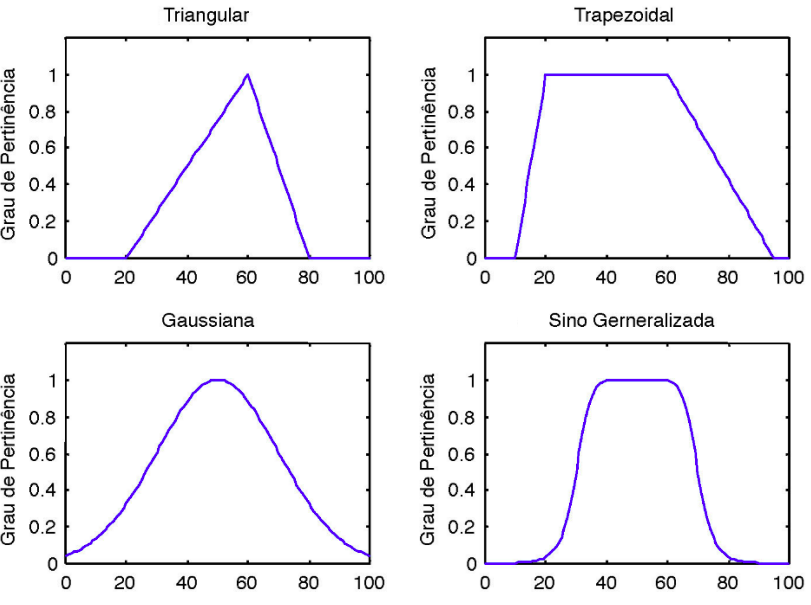
\includegraphics[width=0.5\textwidth]{figs/funcao.png}
    \end{figure}
\end{frame}



\begin{frame}{Variáveis Linguísticas}
\footnotesize
    \begin{block}{}
        \textbf{Definição}: uma variável linguística é uma variável cujo valor não é um número, mas sim uma palavra ou sentença em linguagem natural.
    \end{block}
    \pause
    \begin{itemize}
        \item \textbf{Exemplo:} Velocidade de um carro
        \begin{itemize}
            \item Valores possíveis: \textit{lento}, \textit{moderado}, \textit{rápido}
        \end{itemize}
        \item Cada valor linguístico é associado a um conjunto fuzzy.
    \end{itemize}
    \pause
    \centering
    \begin{tikzpicture}
        % Eixos
        \draw[->] (0, 0) -- (6, 0) node[right] {Velocidade};
        \draw[->] (0, 0) -- (0, 3) node[above] {Grau de Pertinência};

        % Conjuntos fuzzy
        \draw[thick, blue] (0, 0) -- (2, 2) -- (4, 0) node[below] {\footnotesize Lento};
        \draw[thick, red] (2, 0) -- (4, 2) -- (6, 0) node[below] {\footnotesize Moderado};
        \draw[thick, green] (4, 0) -- (6, 2) -- (8, 0) node[below] {\footnotesize Rápido};
    \end{tikzpicture}
\end{frame}

\begin{frame}{Operações Básicas em Conjuntos Fuzzy}
\footnotesize
    \begin{block}{Operações Fundamentais}
        \begin{itemize}
            \item \textbf{Interseção (AND):} \( \mu_{A \cap B}(x) = \min(\mu_A(x), \mu_B(x)) \)
            \item \textbf{União (OR):} \( \mu_{A \cup B}(x) = \max(\mu_A(x), \mu_B(x)) \)
            \item \textbf{Complemento (NOT):} \( \mu_{\neg A}(x) = 1 - \mu_A(x) \)
        \end{itemize}
    \end{block}
    \centering
    \begin{tikzpicture}
        % Eixos
        \draw[->] (0, 0) -- (6, 0) node[right] {$x$};
        \draw[->] (0, 0) -- (0, 3) node[above] {$\mu(x)$};

        % Conjunto A
        \draw[thick, blue] (0, 0) -- (2, 2) -- (4, 0) node[below] {\footnotesize A};

        % Conjunto B
        \draw[thick, red] (1, 0) -- (3, 2) -- (5, 0) node[below] {\footnotesize B};


    \end{tikzpicture}
\end{frame}



\begin{frame}{Operações Básicas em Conjuntos Fuzzy}
\footnotesize
    \begin{block}{Operações Fundamentais}
        \begin{itemize}
            \item \textbf{Interseção (AND):} \( \mu_{A \cap B}(x) = \min(\mu_A(x), \mu_B(x)) \)
            \item \textbf{União (OR):} \( \mu_{A \cup B}(x) = \max(\mu_A(x), \mu_B(x)) \)
            \item \textbf{Complemento (NOT):} \( \mu_{\neg A}(x) = 1 - \mu_A(x) \)
        \end{itemize}
    \end{block}
    \centering
    \begin{tikzpicture}
        % Eixos
        \draw[->] (0, 0) -- (6, 0) node[right] {$x$};
        \draw[->] (0, 0) -- (0, 3) node[above] {$\mu(x)$};

        % Conjunto A
        \draw[thick, blue,opacity=0.1] (0, 0) -- (2, 2) -- (4, 0) node[below] {\footnotesize A};

        % Conjunto B
        \draw[thick, red,opacity=0.1] (1, 0) -- (3, 2) -- (5, 0) node[below] {\footnotesize B};

        % Interseção
        \draw[thick, purple, densely dashed] (1., 0) -- (2.5, 1.5) -- (4, 0) node[below] {\footnotesize $A \cap B$};

    \end{tikzpicture}
\end{frame}


\begin{frame}{Operações Básicas em Conjuntos Fuzzy}
\footnotesize
    \begin{block}{Operações Fundamentais}
        \begin{itemize}
            \item \textbf{Interseção (AND):} \( \mu_{A \cap B}(x) = \min(\mu_A(x), \mu_B(x)) \)
            \item \textbf{União (OR):} \( \mu_{A \cup B}(x) = \max(\mu_A(x), \mu_B(x)) \)
            \item \textbf{Complemento (NOT):} \( \mu_{\neg A}(x) = 1 - \mu_A(x) \)
        \end{itemize}
    \end{block}
    \centering
    \begin{tikzpicture}
        % Eixos
        \draw[->] (0, 0) -- (6, 0) node[right] {$x$};
        \draw[->] (0, 0) -- (0, 3) node[above] {$\mu(x)$};

          % União
        \draw[thick, orange, dotted] (0, 0) -- (2, 2) -- (3, 2) -- (5, 0) node[below] {\footnotesize $A \cup B$};

        % Conjunto A
        \draw[thick, blue,opacity=0.1] (0, 0) -- (2, 2) -- (4, 0) node[below] {\footnotesize A};

        % Conjunto B
        \draw[thick, red,opacity=0.1] (1, 0) -- (3, 2) -- (5, 0) node[below] {\footnotesize B};



    \end{tikzpicture}
\end{frame}


\begin{frame}{Operações Básicas em Conjuntos Fuzzy}
\footnotesize
    \begin{block}{Operações Fundamentais}
        \begin{itemize}
            \item \textbf{Interseção (AND):} \( \mu_{A \cap B}(x) = \min(\mu_A(x), \mu_B(x)) \)
            \item \textbf{União (OR):} \( \mu_{A \cup B}(x) = \max(\mu_A(x), \mu_B(x)) \)
            \item \textbf{Complemento (NOT):} \( \mu_{\neg A}(x) = 1 - \mu_A(x) \)
        \end{itemize}
    \end{block}
    \centering
    \begin{tikzpicture}
        % Eixos
        \draw[->] (0, 0) -- (6, 0) node[right] {$x$};
        \draw[->] (0, 0) -- (0, 3) node[above] {$\mu(x)$};

        % Conjunto A
        \draw[thick, blue,opacity=0.2] (0, 0) -- (2, 2) -- (4, 0) node[below] {\footnotesize A};

        % Conjunto B
        \draw[thick, red,opacity=0.2] (1, 0) -- (3, 2) -- (5, 0) node[below] {\footnotesize B};


        % Complemento de A
        \draw[thick, green, dash dot] (0, 2) -- (2, 0) -- (4, 2) node[below] {\footnotesize $\neg A$};
    \end{tikzpicture}
\end{frame}

\begin{frame}{Normas e Conormas (T-norms e T-conorms)}
\footnotesize
    \begin{block}{Definição}
        \begin{itemize}
            \item \textbf{T-norms (Normas triangulares):} Modelam a operação de conjunção (AND) em lógica fuzzy.
            \item \textbf{T-conorms (Conormas triangulares):} Modelam a operação de disjunção (OR) em lógica fuzzy.
        \end{itemize}
    \end{block}
    \pause
    \begin{block}{Propriedades}
        \begin{itemize}
            \item \textbf{T-norm:} Monotonicidade, comutatividade, associatividade, identidade em 1.
            \item \textbf{T-conorm:} Monotonicidade, comutatividade, associatividade, identidade em 0.
        \end{itemize}
    \end{block}
    \pause
    \centering
    \begin{itemize}
        \item \textbf{Exemplo de T-norm:} \( \min(\mu_A(x), \mu_B(x)) \)
        \item \textbf{Exemplo de T-conorm:} \( \max(\mu_A(x), \mu_B(x)) \)
    \end{itemize}
\end{frame}

% \begin{frame}{Questão}
% \footnotesize
% Considere os seguintes subconjuntos fuzzy \( A(x) \) e \( B(x) \):

% \[
% A(x) =
% \begin{cases}
% x & \text{se } x \in [0, 1], \\
% -x + 3 & \text{se } x \in [1, 3], \\
% 0 & \text{caso contrário}.
% \end{cases}
% \]

% \[
% B(x) =
% \begin{cases}
% 2x & \text{se } x \in [0, 1], \\
% 1 & \text{se } x \in [1, 2], \\
% -2x + 6 & \text{se } x \in [2, 3], \\
% 0 & \text{caso contrário}.
% \end{cases}
% \]

% \textbf{Questão:}
% \begin{enumerate}
%     \item Calcule a interseção fuzzy \( A(x) \cap B(x) \) usando \( \mu_{A \cap B}(x) = \min(A(x), B(x)) \).
%     \item Esboce o gráfico da interseção \( A(x) \cap B(x) \).
% \end{enumerate}
% \end{frame}

% \begin{frame}{Dicas para Resolução}
% \textbf{Passos para resolver:}
% \begin{itemize}
%     \item Identifique os intervalos em que \( A(x) \) e \( B(x) \) estão definidos.
%     \item Para cada intervalo, calcule \( \min(A(x), B(x)) \).
%     \item Combine os resultados para formar a função \( A(x) \cap B(x) \).
%     \item Esboce o gráfico final.
% \end{itemize}
% \end{frame}

% \begin{frame}{Passo 1: Identificação dos Intervalos}
% \textbf{Intervalos relevantes:}
% \begin{itemize}
%     \item \( x \in [0, 1]: \)
%     \[
%     A(x) = x, \quad B(x) = 2x.
%     \]
%     \item \( x \in [1, 2]: \)
%     \[
%     A(x) = -x + 3, \quad B(x) = 1.
%     \]
%     \item \( x \in [2, 3]: \)
%     \[
%     A(x) = -x + 3, \quad B(x) = -2x + 6.
%     \]
% \end{itemize}

% \textbf{Fórmula da interseção:}
% \[
% \mu_{A \cap B}(x) = \min(A(x), B(x)).
% \]
% \end{frame}

% \begin{frame}{Passo 2: Cálculo em Cada Intervalo}
% \footnotesize
% \textbf{Cálculos:}
% \begin{itemize}
%     \item Para \( x \in [0, 1]: \)
%     \[
%     A(x) = x, \quad B(x) = 2x.
%     \]
%     \[
%     \mu_{A \cap B}(x) = \min(x, 2x) = x, \text{ pois } x \leq 2x \text{ nesse intervalo}.
%     \]

%     \item Para \( x \in [1, 2]: \)
%     \[
%     A(x) = -x + 3, \quad B(x) = 1.
%     \]
%     \[
%     \mu_{A \cap B}(x) = \min(-x + 3, 1).
%     \]

%     \item Para \( x \in [2, 3]: \)
%     \[
%     A(x) = -x + 3, \quad B(x) = -2x + 6.
%     \]
%     \[
%     \mu_{A \cap B}(x) = \min(-x + 3, -2x + 6).
%     \]
% \end{itemize}
% \end{frame}

% \begin{frame}{Passo 3: Resultados da Interseção}
% \textbf{Função resultante:}
% \[
% \mu_{A \cap B}(x) =
% \begin{cases}
% x & \text{se } x \in [0, 1], \\
% \min(-x + 3, 1) & \text{se } x \in [1, 2], \\
% \min(-x + 3, -2x + 6) & \text{se } x \in [2, 3], \\
% 0 & \text{caso contrário}.
% \end{cases}
% \]

% \textbf{Simplificando:}
% \begin{itemize}
%     \item Para \( x \in [0, 1]: \) \( \mu_{A \cap B}(x) = x \).
%     \item Para \( x \in [1, 2]: \) \( \mu_{A \cap B}(x) = -x + 3 \) (pois \( -x + 3 \leq 1 \)).
%     \item Para \( x \in [2, 3]: \) \( \mu_{A \cap B}(x) = -x + 3 \) (pois \( -x + 3 \leq -2x + 6 \)).
% \end{itemize}
% \end{frame}



\begin{frame}{Gráfico da Interseção \(A(x) \cap B(x)\)}
\begin{center}
\begin{tikzpicture}[scale=1.8]
    % Eixos
    \draw[->] (-0.5,0) -- (3.5,0) node[right] {\(x\)};
    \draw[->] (0,-0.5) -- (0,1.5) node[above] {\(\mu(x)\)};

    % Interseção A(x) ∩ B(x)
    \draw[green, thick] (0,0) -- (1,1) -- (2,1) -- (3,0) node[right] {\(A(x) \cap B(x)\)};
\end{tikzpicture}
\end{center}
\end{frame}


\begin{frame}{Gráfico dos Conjuntos Fuzzy}
\textbf{Gráfico de \( A(x) \) e \( B(x) \):}
\begin{center}
\begin{tikzpicture}[scale=1.7]
    % Eixos para A(x)
    \draw[->] (-0.5,0) -- (3.5,0) node[right] {\(x\)};
    \draw[->] (0,-0.5) -- (0,2.5) node[above] {\(\mu(x)\)};

    % Conjunto A(x)
    \draw[blue, thick] (0,0) -- (1,1) -- (3,0) node[right] {\(A(x)\)};

    % Conjunto B(x)
    \draw[red, thick] (0,0) -- (1,2) -- (2,1) -- (3,0) node[right] {\(B(x)\)};
\end{tikzpicture}
\end{center}
\end{frame}

\begin{frame}{Gráfico da Interseção}
\textbf{Gráfico da função \( \mu_{A \cap B}(x) \):}
\begin{center}
\begin{tikzpicture}[scale=2]
    % Eixos
    \draw[->] (-0.5,0) -- (3.5,0) node[right] {\(x\)};
    \draw[->] (0,-0.5) -- (0,1.5) node[above] {\(\mu(x)\)};

    % A(x)
    \draw[blue, thick,opacity=0.2] (0,0) -- (1,1) -- (3,0) node[right] {\(A(x)\)};

    % B(x)
    \draw[red, thick,opacity=0.2] (0,0) -- (1,2) -- (2,1) -- (3,0) node[right] {\(B(x)\)};

    % Interseção
    \draw[green, thick] (0,0) -- (1,1) -- (2,1) -- (3,0) node[right] {\(A(x) \cap B(x)\)};
\end{tikzpicture}
\end{center}
\end{frame}

\section{Inferência Fuzzy}
\begin{frame}
\centering
\Huge
\textbf{Inferência\\Fuzzy}
\end{frame}
\subsection{Regras Fuzzy}
\footnotesize
\begin{frame}{Inferência Fuzzy e Regras Fuzzy}
    \begin{block}{Inferência Fuzzy}
        O processo de inferência fuzzy é usado para derivar conclusões a partir de regras fuzzy aplicadas a dados de entrada imprecisos ou incertos.
    \end{block}
    \pause
    \begin{block}{Regras Fuzzy}
        Regras fuzzy são declaradas na forma de sentenças condicionais:
        \begin{itemize}
            \item \textbf{Forma geral:} \textit{SE} antecedente \textit{ENTÃO} consequente
            \item \textbf{Exemplo:} \textit{SE temperatura é alta ENTÃO velocidade do ventilador é alta}
        \end{itemize}
    \end{block}
    \pause
    \begin{itemize}
        \item Regras fuzzy utilizam variáveis linguísticas e suas funções de pertinência para determinar resultados.
        \item A agregação de regras permite combinar múltiplas condições.
    \end{itemize}
    \pause
    \centering
    \begin{tikzpicture}
        % Fluxo da inferência fuzzy
        \node[draw, rectangle, rounded corners, align=center] (input) at (0, 0) {Entradas Fuzzy};
        \node[draw, rectangle, rounded corners, align=center, right=of input] (rules) {Base de Regras Fuzzy};
        \node[draw, rectangle, rounded corners, align=center, right=of rules] (output) {Saídas Fuzzy};

        \draw[->] (input) -- (rules);
        \draw[->] (rules) -- (output);
    \end{tikzpicture}
\end{frame}
\subsection{Sistemas de Inferência Fuzzy}
\begin{frame}{Sistemas de Inferência Fuzzy}
    \begin{block}{Método de Mamdani}

        \begin{itemize}
            \item Um dos métodos mais usados para inferência fuzzy.
            \item As saídas fuzzy são obtidas por um processo de agregação e defuzzificação.
            \item Adequado para sistemas onde as regras são interpretáveis e compreensíveis.
        \end{itemize}
    \end{block}
    \begin{block}{Exemplo de Regras de Mamdani}
        \begin{itemize}
            \item SE temperatura é alta ENTÃO ventilador é rápido.
            \item SE temperatura é baixa ENTÃO ventilador é lento.
        \end{itemize}
    \end{block}
\end{frame}

\begin{frame}{Método de Sugeno}
    \begin{block}{Características principais}

        \begin{itemize}
            \item Baseado em expressões matemáticas ou funções lineares.
            \item A saída fuzzy é convertida diretamente em um valor numérico, sem defuzzificação.
            \item Adequado para sistemas complexos e onde é necessário controle preditivo.
        \end{itemize}
    \end{block}
    \begin{block}{Exemplo de Regras de Sugeno}
        \begin{itemize}
            \item SE temperatura é alta ENTÃO velocidade = 5 + 2\(temp\)
            \item SE temperatura é baixa ENTÃO velocidade = 1 + 0.5\(temp\)
        \end{itemize}
    \end{block}
\end{frame}

\begin{frame}{Comparação entre Mamdani e Sugeno}
    \begin{block}{Diferenças principais}
        \begin{itemize}
            \item \textbf{Mamdani:}
                \begin{itemize}
                    \item Foco em interpretabilidade.
                    \item Saída é uma função fuzzy que requer defuzzificação.
                \end{itemize}
            \item \textbf{Sugeno:}
                \begin{itemize}
                    \item Foco em precisão e simplicidade computacional.
                    \item Saída é numérica, sem necessidade de defuzzificação.
                \end{itemize}
        \end{itemize}
    \end{block}
    \begin{block}{Aplicações}
        \begin{itemize}
            \item \textbf{Mamdani:} Sistemas de suporte à decisão, controle de dispositivos como ventiladores e condicionadores de ar.
            \item \textbf{Sugeno:} Controle avançado de sistemas complexos, como robótica e automação industrial.
        \end{itemize}
    \end{block}
\end{frame}

\subsection{Agregação e Defuzzificação}
\footnotesize
\begin{frame}{}
    \begin{block}{Agregação}
        \begin{itemize}
            \item Combina as saídas fuzzy de todas as regras aplicáveis para formar um único conjunto fuzzy.
            \item Métodos comuns de agregação:
            \begin{itemize}
                \item União: \( \mu_{agregado}(x) = \max(\mu_{regra1}(x), \mu_{regra2}(x), \ldots) \)
                \item Soma: \( \mu_{agregado}(x) = \sum \mu_{regra_i}(x) \)
            \end{itemize}
        \end{itemize}
    \end{block}
    \pause
    \begin{block}{Defuzzificação}
        \begin{itemize}
            \item Converte o conjunto fuzzy agregado em um valor numérico para uso no mundo real.
            \item Métodos comuns de defuzzificação:
            \begin{itemize}
                \item Centro de Gravidade (CoG): \( y = \frac{\int x \cdot \mu(x) dx}{\int \mu(x) dx} \)
                \item Média dos Máximos (MoM): \( y = \text{média}(x \text{ onde } \mu(x) \text{ é máximo}) \)
                \item Altura: \( y = \sum \mu(x_i) \cdot x_i / \sum \mu(x_i) \)
            \end{itemize}
        \end{itemize}
    \end{block}
\end{frame}

\section{Sistemas de Controle Fuzzy}
\begin{frame}
\centering
\Huge
\textbf{Sistemas\\de\\Controle Fuzzy}
\end{frame}
\subsection{Controladores Fuzzy}

\begin{frame}{Controladores Fuzzy}

    \begin{block}{Definição}
        Um controlador fuzzy é um sistema que utiliza lógica fuzzy para determinar as ações de controle baseadas em entradas incertas ou imprecisas.
    \end{block}

\end{frame}

\begin{frame}{Componentes de um Controlador Fuzzy}
    \begin{itemize}
            \item \textbf{Fuzzificação:}
            \begin{itemize}
                \item Transforma as entradas nítidas (crisp) em valores fuzzy.
                \item Usa funções de pertinência para determinar o grau de pertencimento das entradas aos conjuntos fuzzy definidos.
            \end{itemize}
            \item \textbf{Inferência:}
            \begin{itemize}
                \item Aplica regras fuzzy para avaliar as condições e determinar as saídas fuzzy correspondentes.
                \item Utiliza operadores lógicos fuzzy (e.g., AND, OR) para combinar as regras.
            \end{itemize}

        \end{itemize}
 \end{frame}

 \begin{frame}{Componentes de um Controlador Fuzzy}
    \begin{itemize}
            \item \textbf{Defuzzificação:}
            \begin{itemize}
                \item Converte as saídas fuzzy em um valor nítido (crisp) para aplicação no sistema controlado.
                \item Métodos comuns incluem:
                \begin{itemize}
                    \item Centro de Gravidade (CoG): Proporciona equilíbrio considerando toda a área do conjunto fuzzy agregado.
                    \item Média dos Máximos (MoM): Usa o valor médio dos pontos com grau de pertinência máximo.
                \end{itemize}
            \end{itemize}
        \end{itemize}
 \end{frame}

\begin{frame}{Componentes de um Controlador Fuzzy}
    \begin{block}{Exemplo de Aplicação}
        \begin{itemize}
            \item Controle de temperatura: SE temperatura é alta ENTÃO potência do ar-condicionado é alta.
            \item Controle de velocidade: SE distância do carro da frente é pequena ENTÃO velocidade é baixa.
        \end{itemize}
    \end{block}
\end{frame}

\begin{frame}{Aprofunde-se}
    \begin{alertblock}{Consulte sempre o Material Didático}
        Os slides são um guia didático. Para teoria completa, fórmulas e demonstrações, acesse o \textbf{Módulo 5} e os \textbf{notebooks Colab}.
    \end{alertblock}
    \begin{itemize}
        \item \textbf{Módulo 5:} Redes Neurais, Deep Learning, Computação Evolutiva, Fuzzy, AutoML
        \item \textbf{Colab:} logicaFuzzy.ipynb
        \item \faGithub\ \url{https://github.com/eltonsarmanho}
    \end{itemize}
\end{frame}

\section{Redes Neurais}
\begin{frame}
\centering
\Huge
\textbf{Redes \\ Neurais}
\end{frame}

\begin{frame}
\frametitle{Objetivos da Apresentação}
\begin{itemize}
    \item Explorar as características fundamentais das Redes Neurais Artificiais (RNAs).
    \item Compreender o funcionamento básico de uma RNA.
    \item Analisar as principais arquiteturas de RNAs disponíveis.
    \item Ilustrar aplicações de RNAs em Reconhecimento de Padrões e Controle.
\end{itemize}
\end{frame}

\begin{frame}
\frametitle{Motivação Biológica}
\framesubtitle{Ideia Central}
\begin{itemize}
    \item Utilizar neurônios biológicos como modelos para neurônios artificiais.
    \item Neurônios biológicos são o elemento fundamental do sistema nervoso.
    \item Existem diversos tipos de neurônios biológicos.
\end{itemize}
\end{frame}

\begin{frame}
\frametitle{Neurônio Biológico}
\begin{itemize}
    \item O cérebro humano é relativamente lento, mas possui alto paralelismo.
    \item Cerca de $10^{11}$ neurônios, cada um operando a aproximadamente 1 KHz.
    \item Cada neurônio pode se conectar com até $10^4$ outros neurônios.
\end{itemize}
\begin{figure}
    \centering
    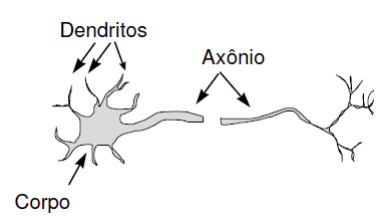
\includegraphics[width=0.5\textwidth]{figs/neuronio.png} % Substitua pelo caminho da sua imagem
    \caption{Representação de um neurônio biológico.}
    \label{fig:neuronio}
\end{figure}
\end{frame}

\begin{frame}
\frametitle{Funcionamento Simplificado de um Neurônio Biológico}
\begin{itemize}
    \item Neurônios podem estar em dois estados:
    \begin{itemize}
        \item \textbf{Ativo ou excitado}: Envia sinais para outros neurônios por meio do axônio e sinapses.
        \item \textbf{Inativo ou inibido}: Não envia sinais.
    \end{itemize}
    \item Sinapses podem ser de dois tipos:
    \begin{itemize}
        \item \textbf{Excitatorias}: Excitam o neurônio receptor.
        \item \textbf{Inibitórias}: Inibem o neurônio receptor.
    \end{itemize}
\end{itemize}
\end{frame}

\begin{frame}
\frametitle{Ativação do Neurônio}
\begin{itemize}
    \item Quando o efeito cumulativo das várias sinapses que chegam a um neurônio excede um valor limite, o neurônio dispara.
    \item O neurônio fica ativo por um período e envia um sinal para outros neurônios.
\end{itemize}
\end{frame}

\begin{frame}
\frametitle{Introdução às Redes Neurais Artificiais}
\begin{itemize}
    \item Redes neurais artificiais são modelos computacionais inspirados no funcionamento do cérebro humano.
    \item Esses modelos são amplamente utilizados em aprendizado de máquina e inteligência artificial.
    \item As redes neurais foram desenvolvidas a partir de contribuições de diversas áreas, como matemática aplicada, estatística e ciência da computação.
\end{itemize}
\end{frame}

\begin{frame}
\frametitle{Origens das Redes Neurais Artificiais}
\begin{itemize}
    \item Os primeiros estudos formais sobre redes neurais artificiais foram realizados por McCulloch e Pitts em 1943.
    \item Eles propuseram um modelo matemático para um neurônio artificial.
    \item Esse modelo era capaz de implementar operações lógicas básicas, como "E" e "OU".
\end{itemize}
\end{frame}

\begin{frame}
\frametitle{Modelo Matemático do Neurônio Artificial}
\begin{itemize}
    \item Um neurônio artificial pode ser representado por uma função \( \eta : \mathbb{R}^n \rightarrow \{0, 1\} \).
    \item A função é definida pela equação:
    \[
    \eta(x) = \chi_{\geq 0} \left[ w^T x - b \right],
    \]
    onde:
    \begin{itemize}
        \item \( w \) é o vetor de pesos,
        \item \( x \) é o vetor de entradas,
        \item \( b \) é o limiar de ativação,
        \item \( \chi_{\geq 0} \) é a função indicadora que retorna 1 se o argumento for maior ou igual a zero, e 0 caso contrário.
    \end{itemize}
\end{itemize}
\end{frame}

\begin{frame}
\frametitle{Aplicações Iniciais}
\begin{itemize}
    \item O modelo de McCulloch e Pitts demonstrou que redes neurais podem resolver problemas de lógica clássica.
    \item Essa descoberta foi um marco inicial para o desenvolvimento de sistemas de inteligência artificial.
    \item Hoje, as redes neurais são aplicadas em diversas áreas, como reconhecimento de padrões, processamento de linguagem natural e visão computacional.
\end{itemize}
\end{frame}

\begin{frame}
\frametitle{Neurônio Artificial}
\begin{itemize}
    \item Um neurônio artificial é uma função \( \eta : \mathbb{R}^n \to \mathbb{R} \).
    \item A função é definida por:
    \[
    \eta(x) = \varphi(w^T x - b),
    \]
    onde:
    \begin{itemize}
        \item \( \varphi \) é a função de ativação,
        \item \( w \) é o vetor de pesos sinápticos,
        \item \( b \) é o viés.
    \end{itemize}
\end{itemize}
\end{frame}
\subsection{Funções de Ativação}
\begin{frame}
\framesubtitle{Funções de Ativação}
\footnotesize
\begin{itemize}
    \item A função de ativação \( \varphi \) determina a saída do neurônio.

\end{itemize}
\begin{block}{Função Limiar}
\[
\chi_{\geq 0}(t) =
\begin{cases}
1, & t \geq 0, \\
0, & t < 0.
\end{cases}
\]
\end{block}
\begin{block}{Função Logística}
\[
\sigma(t) = \frac{1}{(1 + e^{-t})}.
\]
\end{block}
\begin{block}{Função ReLU}
\[
\text{relu}(t) = \max\{0, t\}.
\]
\end{block}
\end{frame}

\begin{frame}
\frametitle{Aplicações das Funções de Ativação}
\begin{itemize}
    \item A função limiar é usada em modelos binários.
    \item A função logística é comum em problemas de classificação.
    \item A função ReLU é amplamente utilizada em redes neurais profundas.
\end{itemize}
\end{frame}

\subsection{Propriedades das Redes Neurais Artificiais}
\begin{frame}
\frametitle{Propriedades das Redes Neurais Artificiais}
\begin{itemize}
    \item As redes neurais artificiais (RNAs) possuem características que as tornam poderosas para diversas aplicações.
    \item Entre as principais propriedades estão: aprendizado, generalização e abstração.
\end{itemize}
\end{frame}

\begin{frame}
\frametitle{Aprendizado}
\begin{itemize}
    \item As RNAs são capazes de modificar seu comportamento com base nos dados de entrada.
    \item Isso permite que elas produzam saídas consistentes e adaptadas ao domínio do problema.
    \item O aprendizado ocorre através da ajuste dos pesos sinápticos durante o treinamento.
\end{itemize}
\end{frame}

\begin{frame}
\frametitle{Generalização}
\begin{itemize}
    \item Após o treinamento, uma RNA pode lidar com pequenas variações nas entradas, como ruídos ou distorções.
    \item Essa capacidade de generalização é essencial para aplicações em cenários do mundo real.
    \item A generalização permite que a rede mantenha um bom desempenho mesmo com dados não vistos durante o treinamento.
\end{itemize}
\end{frame}

\subsection{Arquitetura da Rede Neural}
\begin{frame}
\frametitle{Arquitetura de Redes Neurais}
\begin{itemize}
    \item Os neurônios artificiais são as unidades básicas de processamento em uma rede neural.
    \item Uma rede neural pode ser representada como um grafo direcionado.
    \item Nesse grafo, os vértices correspondem aos neurônios e as arestas indicam conexões entre eles.
\end{itemize}
\end{frame}

\begin{frame}
\frametitle{Topologia da Rede Neural}
\begin{itemize}
    \item A estrutura do grafo é chamada de arquitetura ou topologia da rede neural.
    \item A topologia define como os neurônios estão organizados e conectados.
    \item Existem diferentes tipos de topologias, como redes neurais recorrentes e progressivas.
\end{itemize}
\end{frame}

\begin{frame}
\frametitle{Redes Neurais Recorrentes ou \textit{Feed-backward networks}}
\begin{itemize}
    \item Uma rede neural é dita recorrente quando o grafo associado contém ciclos.
    \item Isso permite que a informação flua em loops, o que é útil para modelar sequências temporais.
    \item Aplicações comuns incluem processamento de linguagem natural e previsão de séries temporais.
\end{itemize}
\end{frame}

\begin{frame}
\frametitle{Redes Neurais Recorrentes ou \textit{Feed-backward networks}}
\begin{figure}
    \centering
    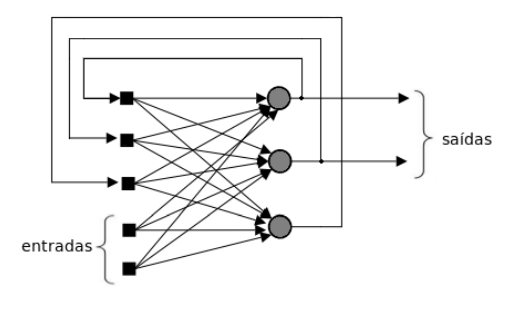
\includegraphics[width=0.7\textwidth]{figs/RedesRecorrentes.png} % Substitua pelo caminho da sua imagem

\end{figure}
\end{frame}



\begin{frame}
\frametitle{Redes Neurais Progressivas ou \textit{Feed-forward networks}}
\begin{itemize}
    \item Uma rede neural é progressiva quando o fluxo de informação segue em uma única direção, sem ciclos.
    \item Também conhecidas como redes feedforward, são amplamente utilizadas em tarefas de classificação e regressão.
    \item Exemplos incluem redes neurais convolucionais (CNNs) e perceptrons multicamadas.
\end{itemize}
\end{frame}

\begin{frame}
\frametitle{Redes Neurais Progressivas ou \textit{Feed-forward networks}}
\begin{figure}
    \centering
    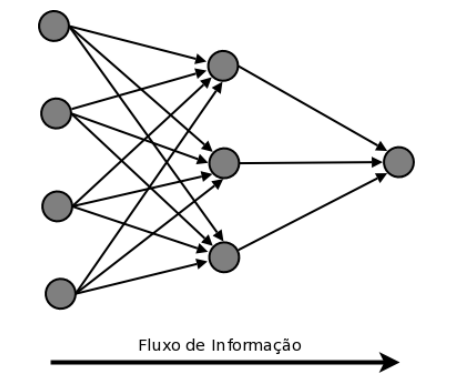
\includegraphics[width=0.4\textwidth]{figs/Feedforwardnetworks.png} % Substitua pelo caminho da sua imagem

\end{figure}
\end{frame}

\subsection{Perceptron}
\begin{frame}
\frametitle{Modelo Matemático do Perceptron}
\begin{itemize}
    \item O Perceptron é uma função \( f: \mathbb{R}^n \to \{0, 1\} \) definida por:
    \[
    f(x) = \begin{cases}
    1, & \text{se } w^T x + b \geq 0, \\
    0, & \text{caso contrário},
    \end{cases}
    \]
    onde:
    \begin{itemize}
        \item \( x \in \mathbb{R}^n \) é o vetor de entrada,
        \item \( w \in \mathbb{R}^n \) é o vetor de pesos,
        \item \( b \in \mathbb{R} \) é o viés.
    \end{itemize}
\end{itemize}
\end{frame}

\begin{frame}
\frametitle{Estrutura do Perceptron}
\begin{figure}
    \centering
    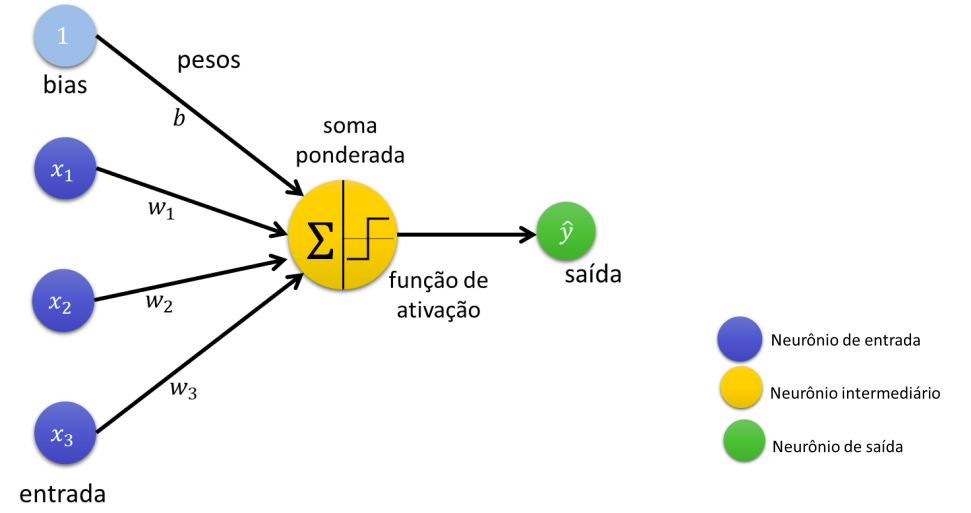
\includegraphics[width=0.8\textwidth]{figs/PERCEPTRON.png} % Substitua pelo caminho da sua imagem

\end{figure}
\end{frame}

\begin{frame}
\frametitle{Estrutura do Perceptron}
\begin{figure}
    \centering
    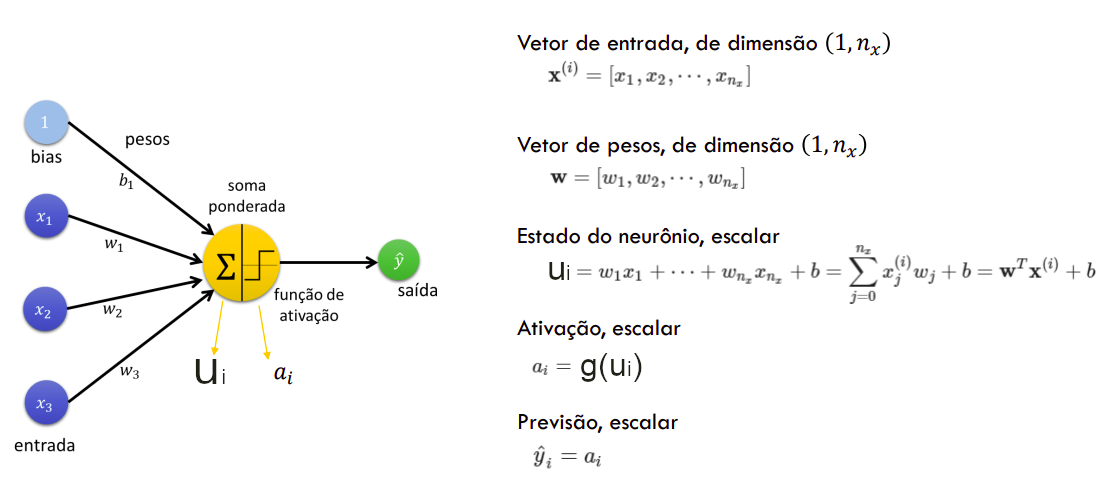
\includegraphics[width=1\textwidth]{figs/PERCEPTRON2.png} % Substitua pelo caminho da sua imagem

\end{figure}
\end{frame}

\begin{frame}
\frametitle{Neurônio que Implementa a Porta OR}
\begin{itemize}
    \item Considere um neurônio com duas entradas \( x_1 \) e \( x_2 \).
    \item Os pesos sinápticos são \( w_1 = 1 \) e \( w_2 = 1 \).
    \item O limiar de ativação é \( \theta = 0,5 \).
    \item A saída \( y \) é dada por:
    \[
    y = \begin{cases}
    1, & \text{se } u \geq 0, \\
    0, & \text{se } u < 0,
    \end{cases}
    \]
    onde \( u = w_1 x_1 + w_2 x_2 - \theta \).
\end{itemize}
\end{frame}

\begin{frame}
\frametitle{Cálculo da Saída para a Porta OR}
\begin{itemize}
    \item A porta OR é definida pela seguinte tabela verdade:
    \begin{table}[]
    \centering
    \begin{tabular}{cc|c}
    \( x_1 \) & \( x_2 \) & \( y \) \\
    \hline
    0 & 0 & 0 \\
    0 & 1 & 1 \\
    1 & 0 & 1 \\
    1 & 1 & 1 \\
    \end{tabular}
    \end{table}
    \item Vamos calcular a saída \( y \) para cada combinação de entradas.
\end{itemize}
\end{frame}

\begin{frame}
\frametitle{Exemplo de Cálculo}
\begin{itemize}
    \item Para \( x_1 = 0 \) e \( x_2 = 0 \):
    \[
    u = (1 \cdot 0) + (1 \cdot 0) - 0,5 = -0,5 \quad \Rightarrow \quad y = 0.
    \]
    \item Para \( x_1 = 0 \) e \( x_2 = 1 \):
    \[
    u = (1 \cdot 0) + (1 \cdot 1) - 0,5 = 0,5 \quad \Rightarrow \quad y = 1.
    \]
    \item Para \( x_1 = 1 \) e \( x_2 = 0 \):
    \[
    u = (1 \cdot 1) + (1 \cdot 0) - 0,5 = 0,5 \quad \Rightarrow \quad y = 1.
    \]
    \item Para \( x_1 = 1 \) e \( x_2 = 1 \):
    \[
    u = (1 \cdot 1) + (1 \cdot 1) - 0,5 = 1,5 \quad \Rightarrow \quad y = 1.
    \]
\end{itemize}
\end{frame}


\begin{frame}
\frametitle{Regra de Treinamento do Perceptron}
\begin{itemize}
    \item A regra de treinamento do Perceptron ajusta os pesos \( w \) e o viés \( b \) para classificar corretamente os dados de treinamento.
    \item Para um conjunto de dados linearmente separável, o algoritmo converge em um número finito de passos.
    \item A atualização dos pesos é dada por:
    \[
    w \leftarrow w + \eta (y_i - \hat{y}_i) x_i,
    \]
    onde:
    \begin{itemize}
        \item \( \eta \) é a taxa de aprendizado,
        \item \( y_i \) é a saída desejada,
        \item \( \hat{y}_i \) é a saída prevista.
    \end{itemize}
\end{itemize}
\end{frame}


\begin{frame}
\frametitle{Neurônio que Implementa a Porta AND}
\begin{itemize}
    \item Considere um neurônio com duas entradas \( x_1 \) e \( x_2 \).
    \item Inicialmente, os pesos sinápticos são \( w_1 = 0,2 \) e \( w_2 = 0,2 \).
    \item O limiar de ativação é \( \theta = 0,5 \).
    \item A saída \( y \) é dada por:
    \[
    y = \begin{cases}
    1, & \text{se } u \geq 0, \\
    0, & \text{se } u < 0,
    \end{cases}
    \]
    onde \( u = w_1 x_1 + w_2 x_2 - \theta \).
\end{itemize}
\end{frame}

\begin{frame}
\frametitle{Regra de Atualização dos Pesos}
\begin{itemize}
    \item A regra de atualização dos pesos é dada por:
    \[
    w_i \leftarrow w_i + \eta (y_{\text{esperado}} - y_{\text{calculado}}) x_i,
    \]
    onde:
    \begin{itemize}
        \item \( \eta \) é a taxa de aprendizado (vamos usar \( \eta = 0,1 \)),
        \item \( y_{\text{esperado}} \) é a saída desejada,
        \item \( y_{\text{calculado}} \) é a saída calculada pelo neurônio.
    \end{itemize}
\end{itemize}
\end{frame}

\begin{frame}
\frametitle{Passo 1: \( x_1 = 1 \), \( x_2 = 1 \)}
\begin{itemize}
    \item Saída esperada: \( y_{\text{esperado}} = 1 \).
    \item Cálculo de \( u \):
    \[
    u = (0,2 \cdot 1) + (0,2 \cdot 1) - 0,5 = -0,1 \quad \Rightarrow \quad y = 0.
    \]
    \item Erro: \( y_{\text{esperado}} - y_{\text{calculado}} = 1 - 0 = 1 \).
    \item Atualização dos pesos:
    \[
    w_1 \leftarrow 0,2 + 0,1 \cdot (1-0) \cdot 1 = 0,3,
    \]
    \[
    w_2 \leftarrow 0,2 + 0,1 \cdot (1-0) \cdot 1 = 0,3.
    \]
    \item Novos pesos: \( w_1 = 0,3 \), \( w_2 = 0,3 \).
\end{itemize}
\end{frame}

\begin{frame}
\frametitle{Passo 1.1: \( x_1 = 1 \), \( x_2 = 1 \)}
\begin{itemize}
    \item Saída esperada: \( y_{\text{esperado}} = 1 \).
    \item Cálculo de \( u \):
    \[
    u = (0,3 \cdot 1) + (0,3 \cdot 1) - 0,5 = 0,1 \quad \Rightarrow \quad y = 1.
    \]
    \item Erro: \( y_{\text{esperado}} - y_{\text{calculado}} = 1 - 1 = 0 \).
   \item Não há atualização dos pesos.
\end{itemize}
\end{frame}

\begin{frame}
\frametitle{Passo 2: \( x_1 = 1 \), \( x_2 = 0 \)}
\begin{itemize}
    \item Saída esperada: \( y_{\text{esperado}} = 0 \).
    \item Cálculo de \( u \):
    \[
    u = (0,3 \cdot 1) + (0,3 \cdot 0) - 0,5 = -0,2 \quad \Rightarrow \quad y = 0.
    \]
    \item Erro: \( y_{\text{esperado}} - y_{\text{calculado}} = 0 - 0 = 0 \).
    \item Não há atualização dos pesos.
\end{itemize}
\end{frame}

\begin{frame}
\frametitle{Passo 3: \( x_1 = 0 \), \( x_2 = 1 \)}
\begin{itemize}
    \item Saída esperada: \( y_{\text{esperado}} = 0 \).
    \item Cálculo de \( u \):
    \[
    u = (0,3 \cdot 0) + (0,3 \cdot 1) - 0,5 = -0,2 \quad \Rightarrow \quad y = 0.
    \]
    \item Erro: \( y_{\text{esperado}} - y_{\text{calculado}} = 0 - 0 = 0 \).
    \item Não há atualização dos pesos.
\end{itemize}
\end{frame}

\begin{frame}
\frametitle{Passo 4: \( x_1 = 0 \), \( x_2 = 0 \)}
\begin{itemize}
    \item Saída esperada: \( y_{\text{esperado}} = 0 \).
    \item Cálculo de \( u \):
    \[
    u = (0,3 \cdot 0) + (0,3 \cdot 0) - 0,5 = -0,5 \quad \Rightarrow \quad y = 0.
    \]
    \item Erro: \( y_{\text{esperado}} - y_{\text{calculado}} = 0 - 0 = 0 \).
    \item Não há atualização dos pesos.
\end{itemize}
\end{frame}

\begin{frame}
\frametitle{Função de Ativação}
\begin{itemize}
    \item A função de ativação \( \varphi: \mathbb{R} \to \mathbb{R} \) é aplicada à saída de um neurônio artificial.
    \item Ela introduz não linearidade no modelo, permitindo que a rede neural aprenda padrões complexos.
    \item Sem a não linearidade, uma rede neural com múltiplas camadas seria equivalente a uma única transformação linear.
\end{itemize}
\end{frame}

\begin{frame}
\frametitle{Importância da Não Linearidade}
\begin{itemize}
    \item Em redes neurais com várias camadas ocultas, a ausência de não linearidade resultaria em uma composição de transformações afins.
    \item Matematicamente, isso pode ser expresso como:
    \[
    f(x) = W_n(W_{n-1}(\dots W_1(x) + b_1) + b_{n-1}) + b_n,
    \]
    onde \( W_i \) são matrizes de pesos e \( b_i \) são vetores de viés.
    \item Sem funções de ativação não lineares, \( f(x) \) seria equivalente a uma única transformação afim:
    \[
    f(x) = W'x + b'.
    \]
\end{itemize}
\end{frame}

\begin{frame}
\frametitle{Exemplos de Funções de Ativação}
\begin{itemize}
    \item \textbf{Função Limiar (Step)}:
    \[
    \varphi(t) = \begin{cases}
    1, & t \geq 0, \\
    0, & t < 0.
    \end{cases}
    \]
    \item \textbf{Função Logística (Sigmoide)}:
    \[
    \sigma(t) = \frac{1}{1 + e^{-t}}.
    \]
    \item \textbf{Função ReLU (Rectified Linear Unit)}:
    \[
    \text{ReLU}(t) = \max(0, t).
    \]
\end{itemize}
\end{frame}

\begin{frame}
\frametitle{Impacto na Aprendizagem}
\begin{itemize}
    \item A não linearidade introduzida pela função de ativação permite que a rede neural modele relações complexas entre entradas e saídas.
    \item Sem funções de ativação não lineares, a rede não seria capaz de aprender funções não lineares, limitando sua aplicabilidade.
    \item A escolha da função de ativação afeta a eficiência do treinamento e a capacidade de generalização do modelo.
\end{itemize}
\end{frame}



\begin{frame}
\frametitle{Limitações do Perceptron}
\begin{itemize}
    \item O Perceptron só pode classificar dados linearmente separáveis.
    \item Ele não consegue resolver problemas não lineares, como o problema do XOR (ou-exclusivo).
    \item Essa limitação foi destacada por Minsky e Papert em 1969, o que levou a um declínio temporário no interesse por redes neurais.
\end{itemize}
\end{frame}
\subsection{RNA}
\begin{frame}
\frametitle{Definição Matemática de uma RNA}
\begin{itemize}
    \item Uma Rede Neural Artificial (RNA) pode ser vista como uma função \( f \) que mapeia um conjunto de dados de entrada \( X \) para um conjunto de saídas \( Y \).
    \item Formalmente, a RNA é uma função:
    \[
    f: \mathbb{R}^{n_x} \to \mathbb{R}^{n_y},
    \]
    onde:
    \begin{itemize}
        \item \( n_x \) é o número de features (entradas),
        \item \( n_y \) é o número de saídas.
    \end{itemize}
\end{itemize}
\end{frame}

\begin{frame}
\frametitle{Representação dos Dados}
\begin{itemize}
    \item Os dados de entrada são representados por uma matriz \( X \in \mathbb{R}^{n_x \times m} \), onde:
    \begin{itemize}
        \item \( n_x \) é o número de features por exemplo,
        \item \( m \) é o número total de exemplos de treinamento.
    \end{itemize}
    \item As saídas desejadas são representadas por uma matriz \( Y \in \mathbb{R}^{n_y \times m} \), onde:
    \begin{itemize}
        \item \( n_y \) é o número de saídas por exemplo.
    \end{itemize}
\end{itemize}
\end{frame}


\begin{frame}
\frametitle{Processo de Aprendizagem}
\begin{itemize}
    \item A principal característica de uma rede neural é sua capacidade de aprender e melhorar o desempenho com base em estímulos externos.
    \item A aprendizagem envolve a atualização da representação interna da rede, ajustando sua arquitetura e os pesos das conexões entre neurônios.
    \item Esse processo permite que a rede desempenhe tarefas específicas de forma mais eficiente ao longo do tempo.
\end{itemize}
\end{frame}

\begin{frame}
\frametitle{Atualização da Representação Interna}
\begin{itemize}
    \item A aprendizagem ocorre por meio da modificação da arquitetura da rede e do ajuste dos pesos sinápticos.
    \item As regras de aprendizagem determinam como os pesos são atualizados em resposta aos erros ou estímulos externos.
    \item Essas regras são essenciais para garantir que a rede se adapte e melhore seu desempenho.
\end{itemize}
\end{frame}

\begin{frame}
\frametitle{Tipos de Regras de Aprendizagem}
\begin{itemize}
    \item \textbf{Aprendizagem por Correção de Erro}:
    \begin{itemize}
        \item Utilizada em treinamento supervisionado.
        \item Os pesos são ajustados com base no erro, que é a diferença entre a saída da rede e o valor esperado.
        \item O erro é minimizado gradualmente ao longo dos ciclos de treinamento.
    \end{itemize}
    \item Outras regras de aprendizagem incluem:
    \begin{itemize}
        \item Aprendizagem Hebbiana,
        \item Aprendizagem Competitiva,
        \item Aprendizagem por Reforço.
    \end{itemize}
\end{itemize}
\end{frame}

\begin{frame}
\frametitle{Aprendizagem por Correção de Erro}
\begin{itemize}
    \item A regra de correção de erro é uma das mais comuns em redes neurais supervisionadas.
    \item O erro é calculado como:
    \[
    \text{Erro} = y_{\text{esperado}} - y_{\text{calculado}}.
    \]
    \item Os pesos são atualizados usando a fórmula:
    \[
    w_i \leftarrow w_i + \eta \cdot \text{Erro} \cdot x_i,
    \]
    onde \( \eta \) é a taxa de aprendizado e \( x_i \) é a entrada.
\end{itemize}
\end{frame}

\begin{frame}
\frametitle{Treinamento da RNA}
\begin{itemize}
    \item Para que a RNA aprenda a mapear \( X \) para \( Y \), ela precisa ser treinada.
    \item O treinamento é um processo de otimização que minimiza uma função de perda \( \mathcal{L} \), que mede a diferença entre as saídas previstas \( \hat{Y} \) e as saídas desejadas \( Y \):
    \[
    \mathcal{L}(Y, \hat{Y}) = \frac{1}{m} \sum_{i=1}^m \| y_i - \hat{y}_i \|^2.
    \]
    \item Durante o treinamento, os parâmetros da RNA (pesos e vieses) são ajustados para minimizar \( \mathcal{L} \).
\end{itemize}
\end{frame}

\begin{frame}
\frametitle{Aprendizado Supervisionado}
\begin{itemize}
    \item O treinamento de uma RNA é tipicamente supervisionado, o que requer um conjunto de dados rotulados \( \{(x_i, y_i)\}_{i=1}^m \).
    \item A cada iteração, a RNA gera uma saída \( \hat{y}_i \) para a entrada \( x_i \).
    \item A diferença entre \( y_i \) e \( \hat{y}_i \) é usada para atualizar os parâmetros da rede via retropropagação.
\end{itemize}
\end{frame}


\subsection{Multi Layer Perceptron}

\begin{frame}
\frametitle{Introdução ao Multi-Layer Perceptron (MLP)}
\begin{itemize}
    \item As limitações do Perceptron simples levaram ao desenvolvimento de redes neurais com múltiplas camadas, como o Adaline e o MLP.
    \item O MLP (Multi-Layer Perceptron) foi proposto por Rumelhart e McClelland em 1986, com base em trabalhos anteriores de Widrow e Hoff (1960).
    \item O MLP é composto por várias camadas de neurônios artificiais, permitindo a modelagem de funções não lineares complexas.
\end{itemize}
\end{frame}

\begin{frame}
\frametitle{Introdução ao MLP}
\begin{itemize}
    \item O Multi-Layer Perceptron (MLP) é uma rede neural artificial com múltiplas camadas de neurônios.
    \item Ele é composto por:
    \begin{itemize}
        \item Uma camada de entrada,
        \item Uma ou mais camadas ocultas,
        \item Uma camada de saída.
    \end{itemize}
    \item A topologia do MLP permite a modelagem de funções não lineares complexas.
\end{itemize}
\end{frame}

\begin{frame}
\frametitle{Topologia do MLP}
\begin{itemize}
    \item A topologia de um MLP é definida pela organização das camadas e pelas conexões entre os neurônios.
    \item Cada camada é composta por um conjunto de neurônios que processam informações e passam os resultados para a camada seguinte.
    \item As conexões entre os neurônios são representadas por pesos sinápticos.
\end{itemize}
\end{frame}

\begin{frame}
\frametitle{Topologia do MLP}
\begin{figure}
    \centering
    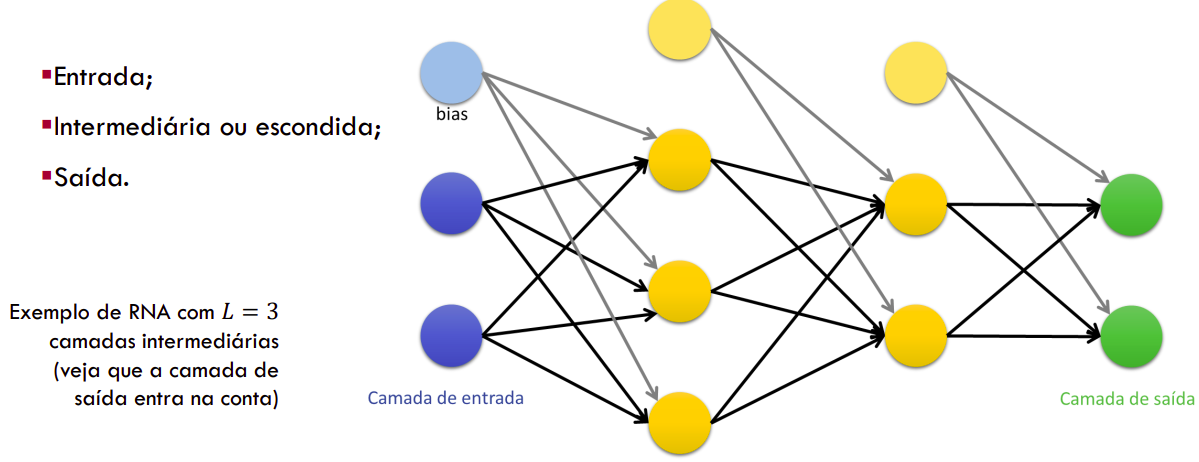
\includegraphics[width=1.05\textwidth]{figs/topologia.png}
\end{figure}
\end{frame}

\begin{frame}
\frametitle{Definição Matemática de uma Camada}
\begin{itemize}
    \item Uma camada de \( m \) neurônios pode ser representada por uma função \( L: \mathbb{R}^n \to \mathbb{R}^m \).
    \item A função de uma camada é dada por:
    \[
    L(x) = \varphi(Wx - b),
    \]
    onde:
    \begin{itemize}
        \item \( W \in \mathbb{R}^{m \times n} \) é a matriz de pesos sinápticos,
        \item \( b \in \mathbb{R}^m \) é o vetor de vieses,
        \item \( \varphi \) é a função de ativação aplicada componente a componente.
    \end{itemize}
\end{itemize}
\end{frame}

\begin{frame}
\frametitle{Camada Densa ou Totalmente Conectada}
\begin{itemize}
    \item Uma camada é chamada de \textbf{densa} ou \textbf{totalmente conectada} se a matriz \( W \) é uma matriz cheia, ou seja, todos os elementos da matriz podem ser diferentes de zero.
    \item Isso significa que cada neurônio na camada recebe entradas de todos os neurônios da camada anterior.
    \item Matematicamente, a densidade da camada é expressa pela estrutura completa da matriz \( W \).
\end{itemize}
\end{frame}

\begin{frame}
\frametitle{Exemplo de MLP com Duas Camadas}
\begin{itemize}
    \item Considere um MLP com duas camadas:
    \begin{itemize}
        \item A primeira camada \( L_1: \mathbb{R}^n \to \mathbb{R}^k \) com função de ativação \( \varphi_1 \).
        \item A segunda camada \( L_2: \mathbb{R}^k \to \mathbb{R}^m \) com função de ativação \( \varphi_2 \).
    \end{itemize}
    \item A função total do MLP é dada por:
    \[
    f(x) = L_2(L_1(x)) = \varphi_2(W_2 \varphi_1(W_1 x - b_1) - b_2).
    \]
    \item Essa composição de camadas permite a modelagem de funções não lineares complexas.
\end{itemize}
\end{frame}

\begin{frame}
\frametitle{Papel das Camadas}
\begin{itemize}
    \item As primeiras camadas (\( L_1, L_2, \ldots \)) atuam como \textbf{extratores de características}, transformando a entrada em representações intermediárias.
    \item As últimas camadas (\( L_{K-1}, L_K \)) realizam a tarefa de aprendizado de máquina, como classificação ou regressão.
    \item A camada \( L_0 \) pode ser incluída como a identidade, representando a entrada original.
\end{itemize}
\end{frame}

\begin{frame}
\frametitle{Redes Neurais Profundas}
\begin{itemize}
    \item Uma rede neural é considerada profunda (\textbf{deep}) quando possui três ou mais camadas (\( K \geq 3 \)).
    \item Redes profundas são capazes de modelar funções altamente não lineares e capturar relações complexas nos dados.
    \item A profundidade da rede permite a extração de características hierárquicas, onde camadas iniciais detectam padrões simples e camadas posteriores combinam esses padrões em representações mais complexas.
\end{itemize}
\end{frame}

\begin{frame}
\frametitle{Exemplo de Rede Profunda}
\begin{itemize}
    \item Considere uma rede com \( K = 4 \) camadas:
    \begin{itemize}
        \item \( L_1: \mathbb{R}^n \to \mathbb{R}^{h_1} \),
        \item \( L_2: \mathbb{R}^{h_1} \to \mathbb{R}^{h_2} \),
        \item \( L_3: \mathbb{R}^{h_2} \to \mathbb{R}^{h_3} \),
        \item \( L_4: \mathbb{R}^{h_3} \to \mathbb{R}^m \).
    \end{itemize}
    \item A função total da rede é:
    \[
    N(x) = L_4(L_3(L_2(L_1(x)))).
    \]
    \item Cada camada aplica uma transformação não linear, permitindo que a rede aprenda representações complexas.
\end{itemize}
\end{frame}

\begin{frame}
\frametitle{Treinamento de Redes Neurais}
\begin{itemize}
    \item O treinamento de uma rede neural (superficial ou profunda) envolve a minimização de uma função de perda.
    \item Em problemas de regressão, a função de perda comum é o \textbf{Erro Quadrático Médio (MSE)}:
    \[
    \text{MSE} = \frac{1}{m} \sum_{i=1}^m (y_i - \hat{y}_i)^2,
    \]
    onde \( y_i \) é o valor esperado e \( \hat{y}_i \) é a saída da rede.
    \item Em problemas de classificação, a função de perda comum é a \textbf{Entropia Cruzada}:
    \[
    \text{Entropia Cruzada} = -\sum_{i=1}^m y_i \log(\hat{y}_i).
    \]
\end{itemize}
\end{frame}

\begin{frame}
\frametitle{Formulação do Problema de Otimização}
\begin{itemize}
    \item O treinamento é formulado como um problema de otimização irrestrito nos parâmetros da rede (pesos \( W \) e vieses \( b \)).
    \item O objetivo é encontrar os parâmetros que minimizam a função de perda:
    \[
    \min_{W, b} \mathcal{L}(W, b),
    \]
    onde \( \mathcal{L} \) é a função de perda.
    \item Devido ao grande número de parâmetros, métodos baseados no gradiente são utilizados.
\end{itemize}
\end{frame}

\begin{frame}
\frametitle{Métodos Baseados no Gradiente}
\begin{itemize}
    \item O gradiente da função de perda em relação aos parâmetros é calculado usando a \textbf{regra da cadeia}.
    \item O gradiente é dado por:
    \[
    \nabla_{W, b} \mathcal{L} = \left( \frac{\partial \mathcal{L}}{\partial W}, \frac{\partial \mathcal{L}}{\partial b} \right).
    \]
    \item O cálculo do gradiente é realizado de forma eficiente usando o algoritmo de retropropagação (\textit{backpropagation}).
\end{itemize}
\end{frame}

\begin{frame}
\frametitle{Algoritmo de Retropropagação}
\begin{itemize}
    \item O algoritmo de retropropagação consiste em duas fases:
    \begin{itemize}
        \item \textbf{Fase Forward}: Calcula a saída da rede para uma dada entrada.
        \item \textbf{Fase Backward}: Propaga o erro da saída para as camadas anteriores, calculando os gradientes.
    \end{itemize}
    \item O gradiente é usado para atualizar os pesos e vieses:
    \[
    W \leftarrow W - \eta \frac{\partial \mathcal{L}}{\partial W}, \quad b \leftarrow b - \eta \frac{\partial \mathcal{L}}{\partial b},
    \]
    onde \( \eta \) é a taxa de aprendizado.
\end{itemize}
\end{frame}

\begin{frame}
\frametitle{Ilustração do Algoritmo de Retropropagação}
Veja o GIF animado:

\end{frame}
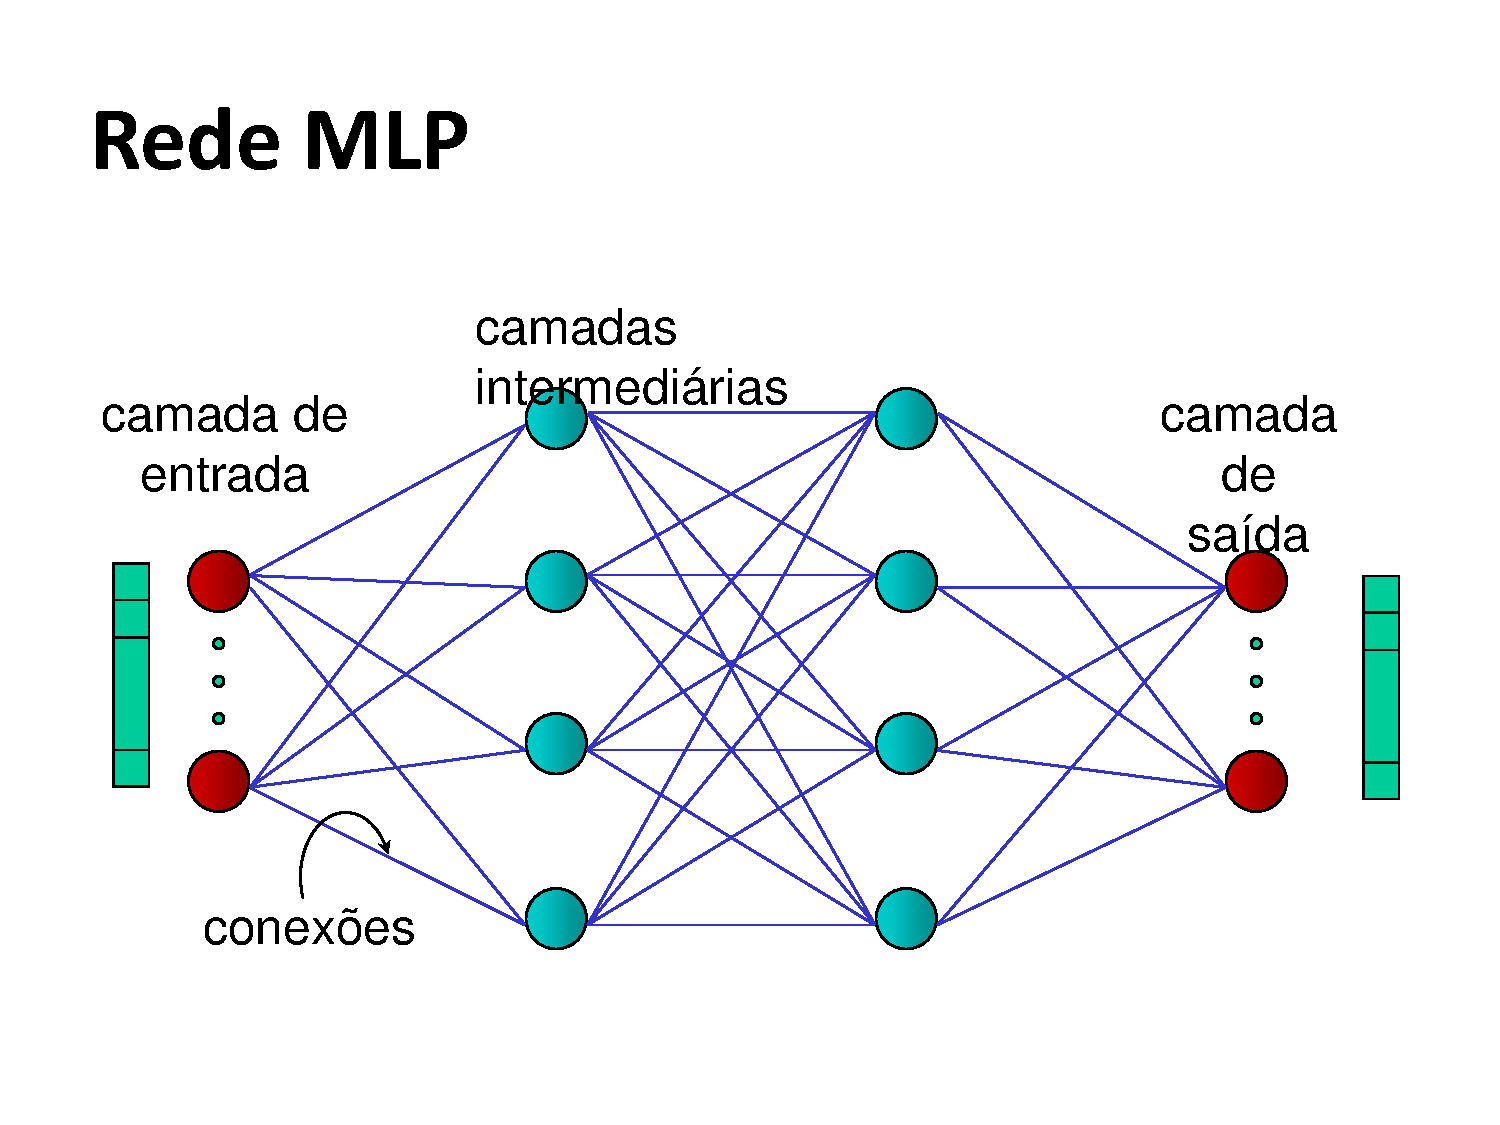
\includepdf[pages=-, frame]{figs/retropropagacao.pdf}

\begin{frame}
\frametitle{Ilustração do Algoritmo de Retropropagação}
\begin{itemize}
    \item A figura abaixo ilustra o fluxo de informações no algoritmo de retropropagação:
    \begin{figure}
        \centering
        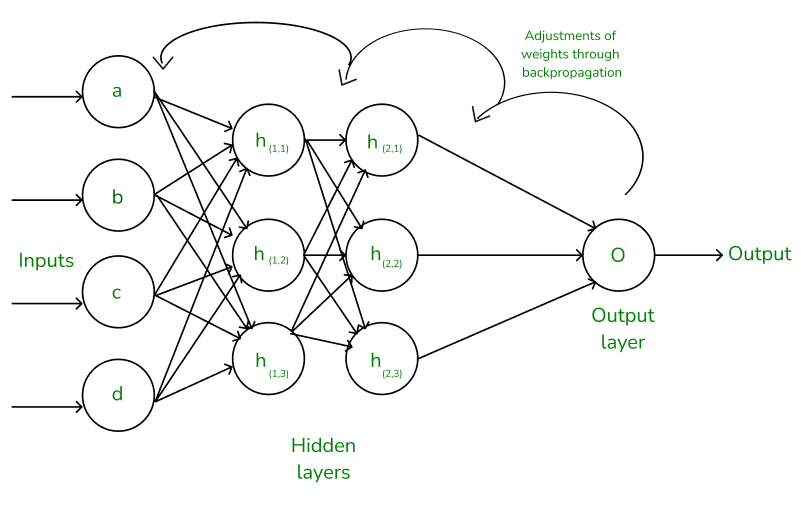
\includegraphics[width=0.65\textwidth]{figs/backpropagation.png} % Substitua pelo caminho da imagem

    \end{figure}
    \item A imagem mostra como o erro é propagado da camada de saída para as camadas anteriores, permitindo o cálculo dos gradientes.
\end{itemize}
\end{frame}

\begin{frame}
\frametitle{Em resumo}
\begin{itemize}
    \item O treinamento de redes neurais é um problema de otimização que busca minimizar uma função de perda.
    \item Métodos baseados no gradiente, como o algoritmo de retropropagação, são essenciais para o treinamento eficiente de redes neurais.
    \item A escolha da função de perda e da taxa de aprendizado é crucial para o desempenho da rede.
\end{itemize}
\end{frame}





%=============================================================
\section{Deep Learning para Mineração de Dados}
%=============================================================

\begin{frame}{Redes Convolucionais (CNN)}
    \begin{columns}
        \column{0.55\textwidth}
        \begin{block}{Convolução}
            Filtro deslizante extrai \textbf{features locais}\\
            $(f * g)[n] = \sum_{k} f[k]\, g[n-k]$
        \end{block}
        \begin{block}{Pooling}
            Reduz dimensionalidade e adiciona \textbf{invariância} a translações\\
            Max Pooling / Average Pooling
        \end{block}
        \column{0.45\textwidth}
        \begin{block}{Aplicações em Mineração de Dados}
            \begin{itemize}
                \item \textbf{Imagens}: extração automática de features visuais
                \item \textbf{Conv1D}: análise de séries temporais e sinais
                \item \textbf{Texto}: CNNs para classificação de documentos
                \item \textbf{Grafos}: Graph CNN para dados relacionais
            \end{itemize}
        \end{block}
        \vspace{0.2cm}
        \centering\tiny \textit{\faArrowRight\ Consulte o Colab para exemplo prático com TensorFlow/Keras}
    \end{columns}
\end{frame}

\begin{frame}{Redes Recorrentes: RNN, LSTM e GRU}
    \begin{columns}
        \column{0.5\textwidth}
        \begin{block}{RNN — Recurrent Neural Network}
            $\mathbf{h}_t = f\!\left(\mathbf{W}_h \mathbf{h}_{t-1} + \mathbf{W}_x \mathbf{x}_t + \mathbf{b}\right)$\\
            Processa \textbf{sequências} com memória de estados anteriores
        \end{block}
        \begin{block}{LSTM (Hochreiter \& Schmidhuber, 1997)}
            Portões \textbf{forget / input / output} controlam o fluxo de informação\\
            Evita o problema de \textit{vanishing gradient}
        \end{block}
        \begin{block}{GRU (Cho et al., 2014)}
            Versão simplificada da LSTM com portões \textbf{reset} e \textbf{update}\\
            Menos parâmetros, performance similar
        \end{block}
        \column{0.5\textwidth}
        \begin{block}{Aplicações em Mineração de Dados}
            \begin{itemize}
                \item \textbf{Séries temporais}: previsão de demanda, clima
                \item \textbf{NLP}: análise de sentimento, tradução
                \item \textbf{Anomalias}: detecção em logs e eventos
                \item \textbf{Recomendação}: modelagem de sequências de itens
            \end{itemize}
        \end{block}
    \end{columns}
\end{frame}



%=============================================================
\section{AutoML e Otimização de Hiperparâmetros}
%=============================================================

% ------------------------------------------------------------------
% HPO Frame 1 — O Problema
% ------------------------------------------------------------------
\begin{frame}{HPO: O Problema de Otimização de Hiperparâmetros}
    \begin{columns}
        \column{0.54\textwidth}
        \begin{block}{Definição Formal}
            \footnotesize
            Encontrar $\lambda^*$ que minimize a perda de validação:
            \[
            \lambda^* = \arg\min_{\lambda \in \Lambda}\,
            \mathcal{L}_{\mathrm{val}}\!\bigl(A(\lambda,\, D_{\mathrm{train}})\bigr)
            \]
            $\Lambda$: espaço de hiperparâmetros;\quad $A$: algoritmo de aprendizado
        \end{block}
        \begin{block}{Parâmetros \textit{vs} Hiperparâmetros}
            \begin{itemize}\footnotesize
                \item \textbf{Parâmetros}: aprendidos durante o treino (pesos $W$, vieses $b$)
                \item \textbf{Hiperparâmetros}: definidos antes do treino:
                      taxa de aprendizado $\eta$, profundidade, dropout, batch size
            \end{itemize}
        \end{block}
        \begin{alertblock}{}\footnotesize
            HPO resolve o desafio de navegar em espaços de alta dimensão com avaliações computacionalmente custosas.
        \end{alertblock}
        \column{0.46\textwidth}
        \centering
        \begin{tikzpicture}[scale=0.82,font=\tiny]
            \draw[->,thick,minegray] (-0.2,0) -- (4.4,0)
                node[right,black] {$\lambda$};
            \draw[->,thick,minegray] (0,-0.2) -- (0,3.4)
                node[above,black] {$\mathcal{L}$};
            \draw[minered,very thick,domain=0.3:4.1,samples=100]
                plot[smooth] (\x,{2.9 - 2.4*exp(-1.4*(\x-2.1)^2)
                     + 0.22*sin(deg(5.5*\x))});
            \draw[minegreen,dashed] (2.1,0)
                node[below,minegreen] {$\lambda^*$} -- (2.1,0.51);
            \fill[minegreen] (2.1,0.51) circle (2.5pt)
                node[above right,minegreen] {ótimo global};
            \fill[mineorange] (3.4,1.8) circle (2.5pt)
                node[right,mineorange] {ótimo local};
            \node[minered,align=left] at (0.8,3.1) {Objetivo\\(não convexa)};
        \end{tikzpicture}
    \end{columns}
\end{frame}

% ------------------------------------------------------------------
% HPO Frame 2 — Grid Search
% ------------------------------------------------------------------
\begin{frame}{Grid Search}
       \begin{block}{Conceito}
            \footnotesize
            Busca exaustiva: define grades de valores e testa \textbf{todas} as combinações com validação cruzada.\\
            Complexidade: $\mathcal{O}(n^k)$, onde $k$ é o número de hiperparâmetros.
        \end{block}
    \begin{columns}
                    \footnotesize

        \column{0.7\textwidth}
     
        \begin{block}{Teoria}
            \begin{itemize}\footnotesize
                \item Conjunto finito de valores por dimensão ($n$ valores, $k$ dimensões)
                \item Total de avaliações: $n^k$ cresce exponencialmente
                \item Seleciona pela menor perda média de validação cruzada
                \item \textbf{Garantia}: encontra o melhor ponto \textit{dentro} da grade definida
            \end{itemize}
        \end{block}
        \begin{alertblock}{Quando usar}
            \begin{itemize}\footnotesize
                \item Espaço pequeno ($\leq 3$ hiperparâmetros, $\leq 5$ valores cada)              
            \end{itemize}
        \end{alertblock}
        \column{0.5\textwidth}
        \centering
        \begin{tikzpicture}[scale=0.50,font=\tiny]
            \draw[->,thick,minegray] (-0.3,0) -- (4.8,0)
                node[right,black] {\small $\eta$ (aprendizado)};
            \draw[->,thick,minegray] (0,-0.3) -- (0,4.5)
                node[above,black] {\small n\_estimators};
            \foreach \xl [count=\xi] in {$10^{-4}$,$10^{-3}$,$10^{-2}$,$10^{-1}$}{
                \node[below,minegray] at (0.9*\xi,0) {\xl};
            }
            \foreach \yl [count=\yi] in {50,100,200,500}{
                \node[left,minegray] at (0,0.9*\yi) {\yl};
            }
            \foreach \xi in {1,...,4}{
                \foreach \yi in {1,...,4}{
                    \fill[mineblue,opacity=0.75] (0.9*\xi, 0.9*\yi) circle (4pt);
                }
            }
            \fill[minered] (0.9*3, 0.9*2) circle (5.5pt)
                node[above right,minered] {melhor};
            \node[mineblue,align=center] at (2.2,4.2)
                {\textbf{16 avaliações} ($4{\times}4$)};
        \end{tikzpicture}
        \vspace{0.1cm}
        \textit{\faArrowRight\ Todos os pontos da grade \\são avaliados igualmente}
    \end{columns}
\end{frame}

% ------------------------------------------------------------------
% HPO Frame 3 — Random Search
% ------------------------------------------------------------------
\begin{frame}{Random Search}
     \begin{block}{Conceito (Bergstra \& Bengio, 2012)}
            \footnotesize
            Amostra aleatória do espaço de hiperparâmetros com distribuições configuráveis: uniforme, log-uniforme, categórica.
        \end{block}
    \begin{columns}
        \column{0.72\textwidth}
       
        \begin{block}{Teoria}
            \begin{itemize}\footnotesize
                \item Hiperparâmetros mais importantes são capturados em mais combinações distintas
                \item Com $n$ avaliações, a probabilidade de encontrar um ponto no top-$p\%$ é:
                $Pr = 1 - \Bigl(1 - \tfrac{p}{100}\Bigr)^{n}$
            \end{itemize}
        \end{block}
        \begin{alertblock}{Quando usar}
            \begin{itemize}\footnotesize
                \item Espaços de alta dimensão ($\geq 4$ hiperparâmetros)
                \item Orçamento de avaliações limitado
                \item Exploração inicial de espaço desconhecido
            \end{itemize}
        \end{alertblock}
        \column{0.3\textwidth}
        \centering
        \begin{tikzpicture}[scale=0.50,font=\tiny]
            \draw[->,thick,minegray] (-0.3,0) -- (4.8,0)
                node[right,black] {\small $\eta$};
            \draw[->,thick,minegray] (0,-0.3) -- (0,4.5)
                node[above,black] {\small n\_estimators};
            \foreach \x/\y in {
                0.4/3.9, 1.0/0.8, 1.2/2.8, 1.7/1.4,
                1.9/3.6, 2.2/0.5, 2.5/2.0, 2.8/3.2,
                3.0/1.1, 3.2/2.7, 3.5/0.3, 3.7/3.5,
                0.7/1.8, 1.5/4.1, 4.2/0.7, 2.7/0.8}{
                \fill[mineorange,opacity=0.80] (\x,\y) circle (3.5pt);
            }
            \fill[minered] (1.7,1.4) circle (5.5pt)
                node[above right,minered] {melhor};
            \node[mineorange,align=center] at (3.4,4.2)
                {\textbf{16 avaliações}\\(espaço contínuo)};
        \end{tikzpicture}
        \vspace{0.1cm}
        \textit{\faArrowRight\ Melhor cobertura do espaço com o mesmo orçamento}
    \end{columns}
\end{frame}

% % ------------------------------------------------------------------
% % HPO Frame 4 — Bayesian Optimization
% % ------------------------------------------------------------------
% \begin{frame}{Otimização Bayesiana}
%      \begin{block}{Conceito}
%             \footnotesize
%             Constrói um \textbf{modelo substituto} (\textit{surrogate}) probabilístico da função objetivo e usa uma \textbf{função de aquisição} para decidir onde avaliar a seguir, equilibrando \textbf{exploração} e \textbf{explotação}.
%         \end{block}
%     \begin{columns}
%         \column{0.7\textwidth}
       
%         \begin{block}{Ciclo iterativo}
%             \footnotesize
%             \begin{enumerate}
%                 \item Avalia $\lambda_i$ e observa $\mathcal{L}(\lambda_i)$
%                 \item Atualiza o surrogate (GP ou TPE)
%                 \item Maximiza a aquisição: $\lambda_{i+1} = \arg\max EI(\lambda)$
%                 \item Repete até o orçamento se esgotar
%             \end{enumerate}
%         \end{block}
%         \begin{alertblock}{Quando usar}
%             \footnotesize Avaliações caras (treino de DNN); espaço contínuo; orçamento $\leq 200$ trials.
%         \end{alertblock}
%         \column{0.48\textwidth}
%         \centering
%         \begin{tikzpicture}[scale=0.75,font=\tiny]
%             \draw[->,thick,minegray] (0,0) -- (5.2,0)
%                 node[right,black] {$\lambda$};
%             \draw[->,thick,minegray] (0,-0.2) -- (0,3.6)
%                 node[above,black] {$\mathcal{L}$};
%             \draw[minered,dashed,thick,domain=0.2:5.0,samples=80]
%                 plot[smooth] (\x,{2.9-2.4*exp(-1.5*(\x-2.5)^2)+0.2*sin(deg(5*\x))});
%             \draw[mineblue,thick,domain=0.2:5.0,samples=60]
%                 plot[smooth] (\x,{2.7-2.1*exp(-1.2*(\x-2.5)^2)});
%             \foreach \x/\y in {0.5/2.5, 1.2/1.8, 2.0/0.95, 3.8/2.4, 4.6/2.8}{
%                 \fill[minegreen] (\x,\y) circle (3pt);
%             }
%             \fill[mineorange] (2.5,0.6) circle (4.5pt)
%                 node[right,mineorange] {próximo (EI máx.)};
%             \draw[minered,dashed,thick] (0.1,3.3) -- (0.65,3.3)
%                 node[right,minered] {Objetivo};
%             \draw[mineblue,thick] (0.1,3.0) -- (0.65,3.0)
%                 node[right,mineblue] {Surrogate};
%             \fill[minegreen] (0.38,2.7) circle (3pt)
%                 node[right,minegreen] {Avaliados};
%             \fill[mineorange] (0.38,2.4) circle (4pt)
%                 node[right,mineorange] {Próximo};
%         \end{tikzpicture}
%         \vspace{0.1cm}
%         \textit{\faArrowRight\ Surrogate guia avaliações para regiões promissoras}
%     \end{columns}
% \end{frame}

% \begin{frame}{Otimização Bayesiana: TPE}
%     \begin{columns}
%         \column{0.55\textwidth}
%         \begin{block}{TPE — Tree-structured Parzen Estimator}
%             \footnotesize
%             O TPE (usado pelo Optuna) modela a distribuição de hiperparâmetros separadamente para os \textbf{bons} e \textbf{maus} resultados:
%             \[
%             \ell(\lambda) = p(\lambda \mid \mathcal{L} < \tau), \quad
%             g(\lambda) = p(\lambda \mid \mathcal{L} \geq \tau)
%             \]
%             A função de aquisição \textbf{Expected Improvement} é proporcional a:
%             \[
%             EI(\lambda) \propto \frac{\ell(\lambda)}{g(\lambda)}
%             \]
%             Favorece regiões onde bons resultados são prováveis e maus resultados são improváveis.
%         \end{block}
%         \begin{block}{Vantagens do TPE}
%             \begin{itemize}\footnotesize
%                 \item Funciona bem com hiperparâmetros condicionais (espaços em árvore)
%                 \item Robusto a hiperparâmetros irrelevantes
%                 \item Mais eficiente que Gaussian Process em alta dimensão
%             \end{itemize}
%         \end{block}
%         \column{0.45\textwidth}
%         \centering
%         \begin{tikzpicture}[scale=0.75,font=\tiny]
%             \draw[->,thick,minegray] (0,0) -- (5.0,0)
%                 node[right,black] {$\lambda$};
%             \draw[->,thick,minegray] (0,-0.1) -- (0,3.4)
%                 node[above,black] {$p(\lambda)$};
%             % l(lambda): good distribution
%             \draw[minegreen,very thick,domain=0.2:4.8,samples=60]
%                 plot[smooth] (\x,{2.0*exp(-3.0*(\x-2.0)^2)});
%             \node[minegreen] at (2.0,2.4) {$\ell(\lambda)$ (bons)};
%             % g(lambda): bad distribution
%             \draw[minered,very thick,domain=0.2:4.8,samples=60]
%                 plot[smooth] (\x,{1.2*exp(-0.8*(\x-3.2)^2)+0.3*exp(-2*(\x-0.8)^2)});
%             \node[minered] at (3.8,1.5) {$g(\lambda)$ (ruins)};
%             % threshold tau
%             \draw[mineorange,dashed] (0,0.5) node[left,mineorange] {$\tau$} -- (4.8,0.5);
%             % next point
%             \draw[mineblue,dashed] (2.0,0) node[below,mineblue] {$\lambda^*$} -- (2.0,2.0);
%         \end{tikzpicture}
%         \vspace{0.2cm}
%         \begin{alertblock}{Quando usar}
%             \footnotesize Optuna usa TPE por padrão — ideal para a maioria dos problemas de HPO em DL e ML.
%         \end{alertblock}
%     \end{columns}
% \end{frame}

% % ------------------------------------------------------------------
% % HPO Frame 5 — Optuna
% % ------------------------------------------------------------------
% \begin{frame}[shrink=5]{Optuna: Framework de HPO}
%     \begin{columns}
%         \column{0.50\textwidth}
%         \begin{block}{Optuna (Akiba et al., 2019)}
%             Framework Python moderno, integra sampler, pruner e visualização.
%             \begin{itemize}\footnotesize
%                 \item \faCheck\ Sampler TPE por padrão (Bayesiano)
%                 \item \faCheck\ Pruning de trials não promissoras (\textit{MedianPruner})
%                 \item \faCheck\ Dashboard visual interativo
%                 \item \faCheck\ Otimização paralela (multi-processo/nó)
%                 \item \faCheck\ \textit{Define-by-run}: espaço de busca dinâmico
%                 \item \faCheck\ Otimização multi-objetivo (Pareto)
%             \end{itemize}
%         \end{block}
%         \begin{block}{Oportunidades de uso}\footnotesize
%             \begin{itemize}
%                 \item Ajuste automático de MLP, CNN, LSTM, XGBoost sem tentativa-erro manual
%                 \item Pipeline AutoML integrado com Scikit-Learn
%                 \item Comparar múltiplos modelos em um único \textit{study}
%                 \item Otimizar acurácia \textit{vs} tempo de inferência simultaneamente
%                 \item Integração com MLflow/W\&B para rastreamento de experimentos
%             \end{itemize}
%         \end{block}
%         \column{0.50\textwidth}
%         \centering
%         \begin{tikzpicture}[
%             box/.style={rectangle,draw=mineblue,fill=mineblue!10,
%                         rounded corners=3pt,minimum width=3.2cm,
%                         minimum height=0.75cm,font=\small\bfseries,
%                         align=center},
%             act/.style={rectangle,draw=mineorange,fill=mineorange!10,
%                          rounded corners=3pt,minimum width=2.6cm,
%                          minimum height=0.65cm,font=\footnotesize,
%                          align=center},
%             arr/.style={-{Stealth[length=5pt]},thick}]
%             \node[box]  (study) at (0, 0.0)  {Criar Study};
%             \node[box]  (sug)   at (0,-1.15) {Sugerir $\lambda$\\(TPE Sampler)};
%             \node[box]  (eval)  at (0,-2.30) {Treinar e Avaliar\\$\mathcal{L}(\lambda)$};
%             \node[box]  (prune) at (0,-3.45) {Pruning?};
%             \node[box]  (rep)   at (0,-4.60) {Reportar Trial};
%             \node[act]  (best)  at (3.4,-4.60) {Melhor\\$\lambda^*$};
%             \node[act]  (dash)  at (3.4,-2.30) {Dashboard\\Optuna};
%             \draw[arr,mineblue]   (study) -- (sug);
%             \draw[arr,mineblue]   (sug)   -- (eval);
%             \draw[arr,mineblue]   (eval)  -- (prune);
%             \draw[arr,mineblue]   (prune) -- (rep);
%             \draw[arr,minered]    (prune.east) -- ++(0.5,0)
%                 node[above right,font=\tiny,minered]{Sim (poda)} |- (sug.east);
%             \draw[arr,mineblue]   (rep.west)  -- ++(-0.7,0)
%                 node[left,font=\tiny,minegray]{loop} |- (sug.west);
%             \draw[arr,mineorange] (rep.east)  -- (best.west);
%             \draw[arr,mineorange] (eval.east) -- (dash.west);
%         \end{tikzpicture}
%         \vspace{0.15cm}
%         \centering\tiny \textit{\faArrowRight\ Colab: experimento Optuna vs Grid Search em dataset real}
%     \end{columns}
% \end{frame}

% \begin{frame}{AutoML: Aprendizado de Máquina Automatizado}
%     \begin{columns}
%         \column{0.5\textwidth}
%         \begin{block}{TPOT}
%             \textbf{Programação Genética} para otimizar automaticamente pipelines de ML\\
%             Evolui combinações de pré-processamento, transformações e modelos
%         \end{block}
%         \begin{block}{Auto-sklearn}
%             \textbf{Bayesian Optimization} + \textit{meta-learning} + \textit{ensemble}\\
%             Aprende de resultados em datasets anteriores (warm start)
%         \end{block}
%         \column{0.5\textwidth}
%         \begin{block}{AutoGluon}
%             \textit{Stacking} multicamadas automático\\
%             Combina múltiplos modelos em estrutura de ensemble hierárquico
%         \end{block}
%         \begin{alertblock}{Consulte}
%             Material Didático Módulo 5 e Colab para experimentos práticos com AutoML e Optuna. Compare Grid Search e Bayesian Optimization em datasets reais.
%         \end{alertblock}
%     \end{columns}
% \end{frame}

%=============================================================
\section{Estado da Arte (2020--2024)}
%=============================================================

\begin{frame}{Transformers para Dados Tabulares}
    \begin{columns}
        \column{0.5\textwidth}
        \begin{block}{FT-Transformer (Gorishniy et al., 2021)}
            \textbf{Feature Tokenizer} + Transformer\\
            Converte features numéricas/categóricas em tokens e aplica atenção
        \end{block}
        \begin{block}{TabPFN (Hollmann et al., 2022)}
            \textbf{Prior-Fitted Network}\\
            Treinado em datasets sintéticos — estado da arte em datasets pequenos\\
            Inferência em milissegundos sem fine-tuning
        \end{block}
        \column{0.5\textwidth}
        \begin{block}{O Grande Debate}
            \begin{itemize}
                \item \faArrowRight\ Transformers atingem resultados \textbf{state-of-the-art} em benchmarks tabulares
                \item \faArrowRight\ Porém \textbf{GBDTs} (XGBoost, LightGBM, CatBoost) ainda dominam em \textbf{eficiência e robustez} no mundo real
                \item \faArrowRight\ Recomendação: comece com GBDT, experimente Transformers se tiver dados suficientes
            \end{itemize}
        \end{block}
    \end{columns}
\end{frame}

\begin{frame}[shrink=5]{Self-Supervised Learning e Redes Generativas}
    \begin{columns}
        \column{0.5\textwidth}
        \begin{block}{SCARF (Bahri et al., 2022)}
            \textbf{Contrastive Learning} para dados tabulares\\
            Aprende representações ricas sem rótulos via corrupção de features\\
            Pré-treino + fine-tuning com poucos exemplos rotulados
        \end{block}
        \begin{block}{Dados Sintéticos Tabulares}
            \begin{itemize}
                \item \textbf{CTGAN}: GAN condicional para tabelas
                \item \textbf{TVAE}: Variational Autoencoder tabular
            \end{itemize}
            Geram dados sintéticos realistas preservando distribuições marginais e correlações
        \end{block}
        \column{0.5\textwidth}
        \begin{block}{Aplicações Práticas}
            \begin{itemize}
                \item \textbf{Balanceamento}: gerar exemplos da classe minoritária
                \item \textbf{Privacidade}: substituir dados sensíveis por sintéticos
                \item \textbf{Data Augmentation}: ampliar datasets pequenos
                \item \textbf{Benchmarking}: criar cenários de teste controlados
            \end{itemize}
        \end{block}
        \reflexao{Dados sintéticos de qualidade podem valer mais do que mais dados reais!}
    \end{columns}
\end{frame}

%=============================================================
% Frame final e Referências
%=============================================================

\begin{frame}{Aprofunde-se no Material Didático}
    \begin{alertblock}{Consulte sempre o Material Didático}
        Os slides são um guia didático. Para teoria completa, fórmulas e demonstrações, acesse o \textbf{Módulo 5 — Material Didático} e os \textbf{notebooks Colab}.
    \end{alertblock}
    \begin{itemize}
        \item \textbf{Módulo 5:} Redes Neurais, Deep Learning, Computação Evolutiva, Fuzzy, AutoML
        \item \textbf{Colab:} Implementações em TensorFlow/Keras, Algoritmo Genético, PSO, Optuna
        \item \faGithub\ \url{https://github.com/eltonsarmanho}
    \end{itemize}
\end{frame}

\begin{frame}{Referências Bibliográficas}
    \begin{thebibliography}{9}
        \bibitem{goodfellow} GOODFELLOW, I.; BENGIO, Y.; COURVILLE, A. \textit{Deep Learning}. MIT Press, 2016.
        \bibitem{geron} GÉRON, A. \textit{Hands-On Machine Learning with Scikit-Learn, Keras, and TensorFlow}. O'Reilly, 2019.
        \bibitem{rumelhart} RUMELHART et al. Learning representations by back-propagating errors. \textit{Nature}, 323, 1986.
        \bibitem{holland} HOLLAND, J. H. \textit{Adaptation in Natural and Artificial Systems}. U. Michigan Press, 1975.
        \bibitem{zadeh} ZADEH, L. Fuzzy sets. \textit{Information and Control}, 8(3):338--353, 1965.
        \bibitem{akiba} AKIBA et al. Optuna: A next-generation hyperparameter optimization framework. \textit{KDD}, 2019.
    \end{thebibliography}
\end{frame}

\end{document}
